% !TeX program = xelatex
\documentclass[UTF8,a4paper,12pt]{ctexart}

\usepackage[margin=2.2cm]{geometry}
\usepackage{graphicx}
\usepackage{booktabs}
\usepackage{float}
\usepackage{subcaption}
\usepackage{amsmath}
\usepackage{amssymb}
\usepackage{xcolor}
\usepackage{listings}
\usepackage{hyperref}

\graphicspath{{./}{outputs/}{outputs/task_lowpass/}{outputs/task_highpass/}}

\hypersetup{
  colorlinks=true,
  linkcolor=blue,
  urlcolor=blue,
  citecolor=blue
}

\lstdefinestyle{py}{
  language=Python,
  basicstyle=\ttfamily\small,
  keywordstyle=\color{blue!70!black},
  commentstyle=\color{green!40!black},
  stringstyle=\color{orange!60!black},
  numbers=left,
  numberstyle=\tiny\color{gray},
  stepnumber=1,
  numbersep=8pt,
  frame=single,
  breaklines=true,
  tabsize=4,
  showstringspaces=false
}

\title{视频图像处理实验报告\\第四次作业：空域滤波与边缘检测}
\author{姓名：\underline{\hspace{3cm}} \quad 学号：\underline{\hspace{3cm}}}
\date{\today}

\begin{document}
\maketitle
\tableofcontents
\newpage

\section{实验目的}
\begin{enumerate}
  \item 掌握空域低通滤波器的基本原理和实现方法。
  \item 比较高斯滤波与中值滤波在不同模板尺寸下的平滑效果。
  \item 掌握常见高通增强与边缘检测方法，包括 Unsharp Masking、Sobel、Laplace 和 Canny。
  \item 结合实验结果分析不同算法的适用场景、优缺点和参数影响。
\end{enumerate}

\section{实验环境与数据}
\subsection{实验环境}
\begin{itemize}
  \item 操作系统：Windows
  \item 编程语言：Python 3
  \item 主要库：NumPy、Pillow、SciPy、Matplotlib、scikit-image、tifffile
\end{itemize}

\subsection{实验数据}
\begin{itemize}
  \item 低通滤波测试图像：\texttt{test1.pgm}、\texttt{test2.tif}
  \item 高通与边缘检测测试图像：\texttt{test3\_corrupt.pgm}、\texttt{test4.tif}
\end{itemize}

\section{实验任务}
根据题目要求，本次实验完成以下内容：
\begin{enumerate}
  \item 用高斯滤波器和中值滤波器平滑 \texttt{test1}、\texttt{test2}，模板大小分别取 $3\times3$、$5\times5$、$7\times7$；
  \item 固定高斯滤波器参数 $\sigma=1.5$，生成不同尺寸的高斯核；
  \item 对 \texttt{test3}、\texttt{test4} 分别进行 Unsharp Masking、Sobel、Laplace、Canny 处理；
  \item 对各方法实验结果进行分析并总结优缺点。
\end{enumerate}

\section{实验原理}
\subsection{高斯滤波}
二维高斯核定义为：
\begin{equation}
G(x,y)=\frac{1}{2\pi\sigma^2}\exp\left(-\frac{x^2+y^2}{2\sigma^2}\right)
\end{equation}
本实验固定 $\sigma=1.5$，分别构造 $3\times3$、$5\times5$、$7\times7$ 模板，并对图像做卷积平滑。高斯滤波适合抑制连续型随机噪声，但会使边缘逐渐模糊。

\subsection{中值滤波}
中值滤波在局部窗口内取中值代替中心像素：
\begin{equation}
\hat{f}(x,y)=\mathrm{median}\{f(i,j)\mid (i,j)\in \mathcal{N}(x,y)\}
\end{equation}
它对脉冲噪声、椒盐噪声更鲁棒，同时比线性平滑更能保边缘。

\subsection{Unsharp Masking}
反锐化掩模通过将原图减去平滑图得到高频分量，再加回原图实现锐化：
\begin{equation}
g(x,y)=f(x,y)+k\left[f(x,y)-f_{blur}(x,y)\right]
\end{equation}
其中 $k>0$ 为增强系数。本实验使用高斯模糊作为 $f_{blur}$。

\subsection{Sobel 边缘检测}
Sobel 通过计算水平和垂直梯度来估计边缘强度：
\begin{equation}
M(x,y)=\sqrt{G_x^2+G_y^2}
\end{equation}
该方法实现简单，但边缘通常较粗，且对噪声较敏感。

\subsection{Laplace 边缘检测}
Laplace 算子属于二阶导数：
\begin{equation}
\nabla^2 f=\frac{\partial^2 f}{\partial x^2}+\frac{\partial^2 f}{\partial y^2}
\end{equation}
它对灰度突变更敏感，能够突出细节，但也更容易放大噪声。

\subsection{Canny 边缘检测}
Canny 先做高斯平滑，再计算梯度，并结合非极大值抑制和双阈值连接得到边缘。其优点是边缘细、连续性较好、抗噪性能较强。

\section{关键代码}
\subsection{高斯核生成}
\begin{lstlisting}[style=py]
def gaussian_kernel(size: int, sigma: float = 1.5) -> np.ndarray:
    radius = size // 2
    y, x = np.mgrid[-radius : radius + 1, -radius : radius + 1]
    kernel = np.exp(-(x**2 + y**2) / (2 * sigma**2))
    kernel /= kernel.sum()
    return kernel
\end{lstlisting}

\subsection{高斯滤波与中值滤波}
\begin{lstlisting}[style=py]
def gaussian_filter_manual(img: np.ndarray, size: int, sigma: float = 1.5) -> np.ndarray:
    kernel = gaussian_kernel(size, sigma)
    filtered = ndimage.convolve(img.astype(np.float32), kernel, mode="reflect")
    return ensure_u8(filtered)

def median_filter(img: np.ndarray, size: int) -> np.ndarray:
    filtered = ndimage.median_filter(img, size=size, mode="reflect")
    return ensure_u8(filtered)
\end{lstlisting}

\subsection{高通和边缘方法}
\begin{lstlisting}[style=py]
def unsharp_mask(img: np.ndarray, sigma: float = 1.5, amount: float = 1.5) -> np.ndarray:
    blurred = ndimage.gaussian_filter(img.astype(np.float32), sigma=sigma, mode="reflect")
    sharpened = img.astype(np.float32) + amount * (img.astype(np.float32) - blurred)
    return ensure_u8(sharpened)

def canny_edges(img: np.ndarray, sigma: float = 1.2) -> np.ndarray:
    edges = feature.canny(img.astype(np.float32) / 255.0, sigma=sigma)
    return (edges.astype(np.uint8) * 255)
\end{lstlisting}

\section{实验结果与分析}
\subsection{高斯核可视化}
\begin{figure}[H]
  \centering
  \begin{subfigure}{0.31\textwidth}
    \centering
    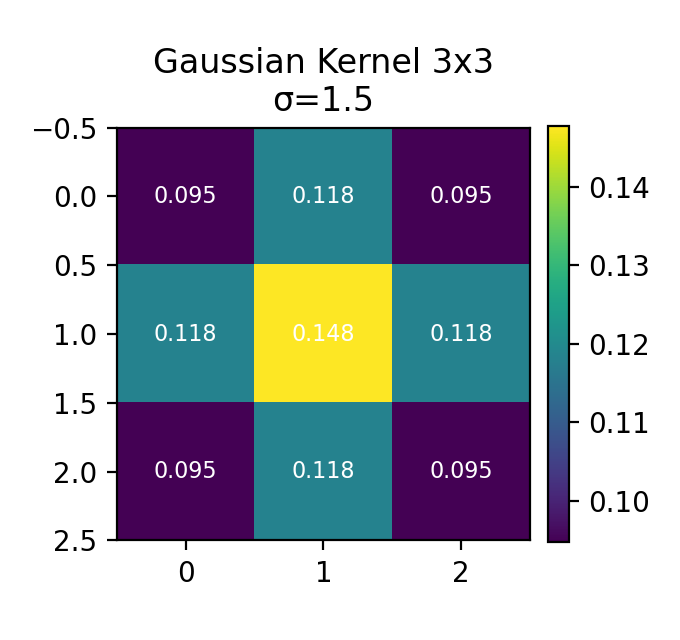
\includegraphics[width=\linewidth]{gaussian_kernel_3x3.png}
    \caption{$3\times3$}
  \end{subfigure}
  \begin{subfigure}{0.31\textwidth}
    \centering
    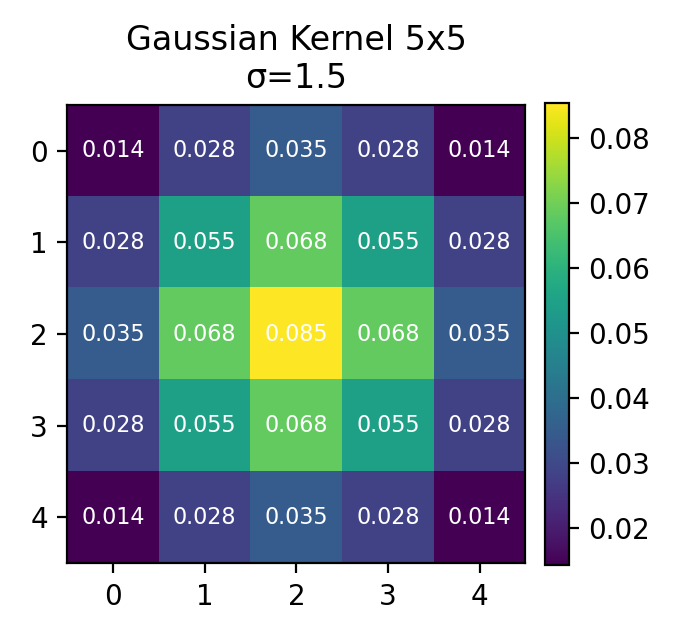
\includegraphics[width=\linewidth]{gaussian_kernel_5x5.png}
    \caption{$5\times5$}
  \end{subfigure}
  \begin{subfigure}{0.31\textwidth}
    \centering
    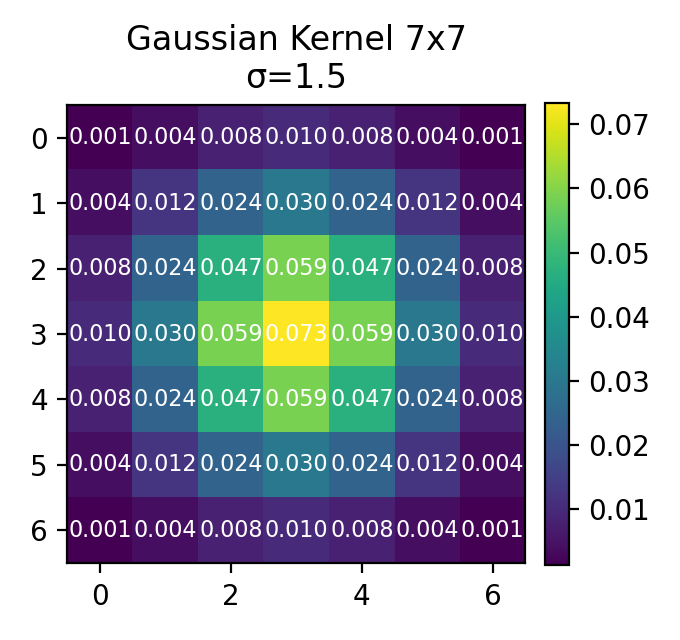
\includegraphics[width=\linewidth]{gaussian_kernel_7x7.png}
    \caption{$7\times7$}
  \end{subfigure}
  \caption{固定 $\sigma=1.5$ 时的高斯核}
\end{figure}

\subsection{低通滤波结果}
\begin{figure}[H]
  \centering
  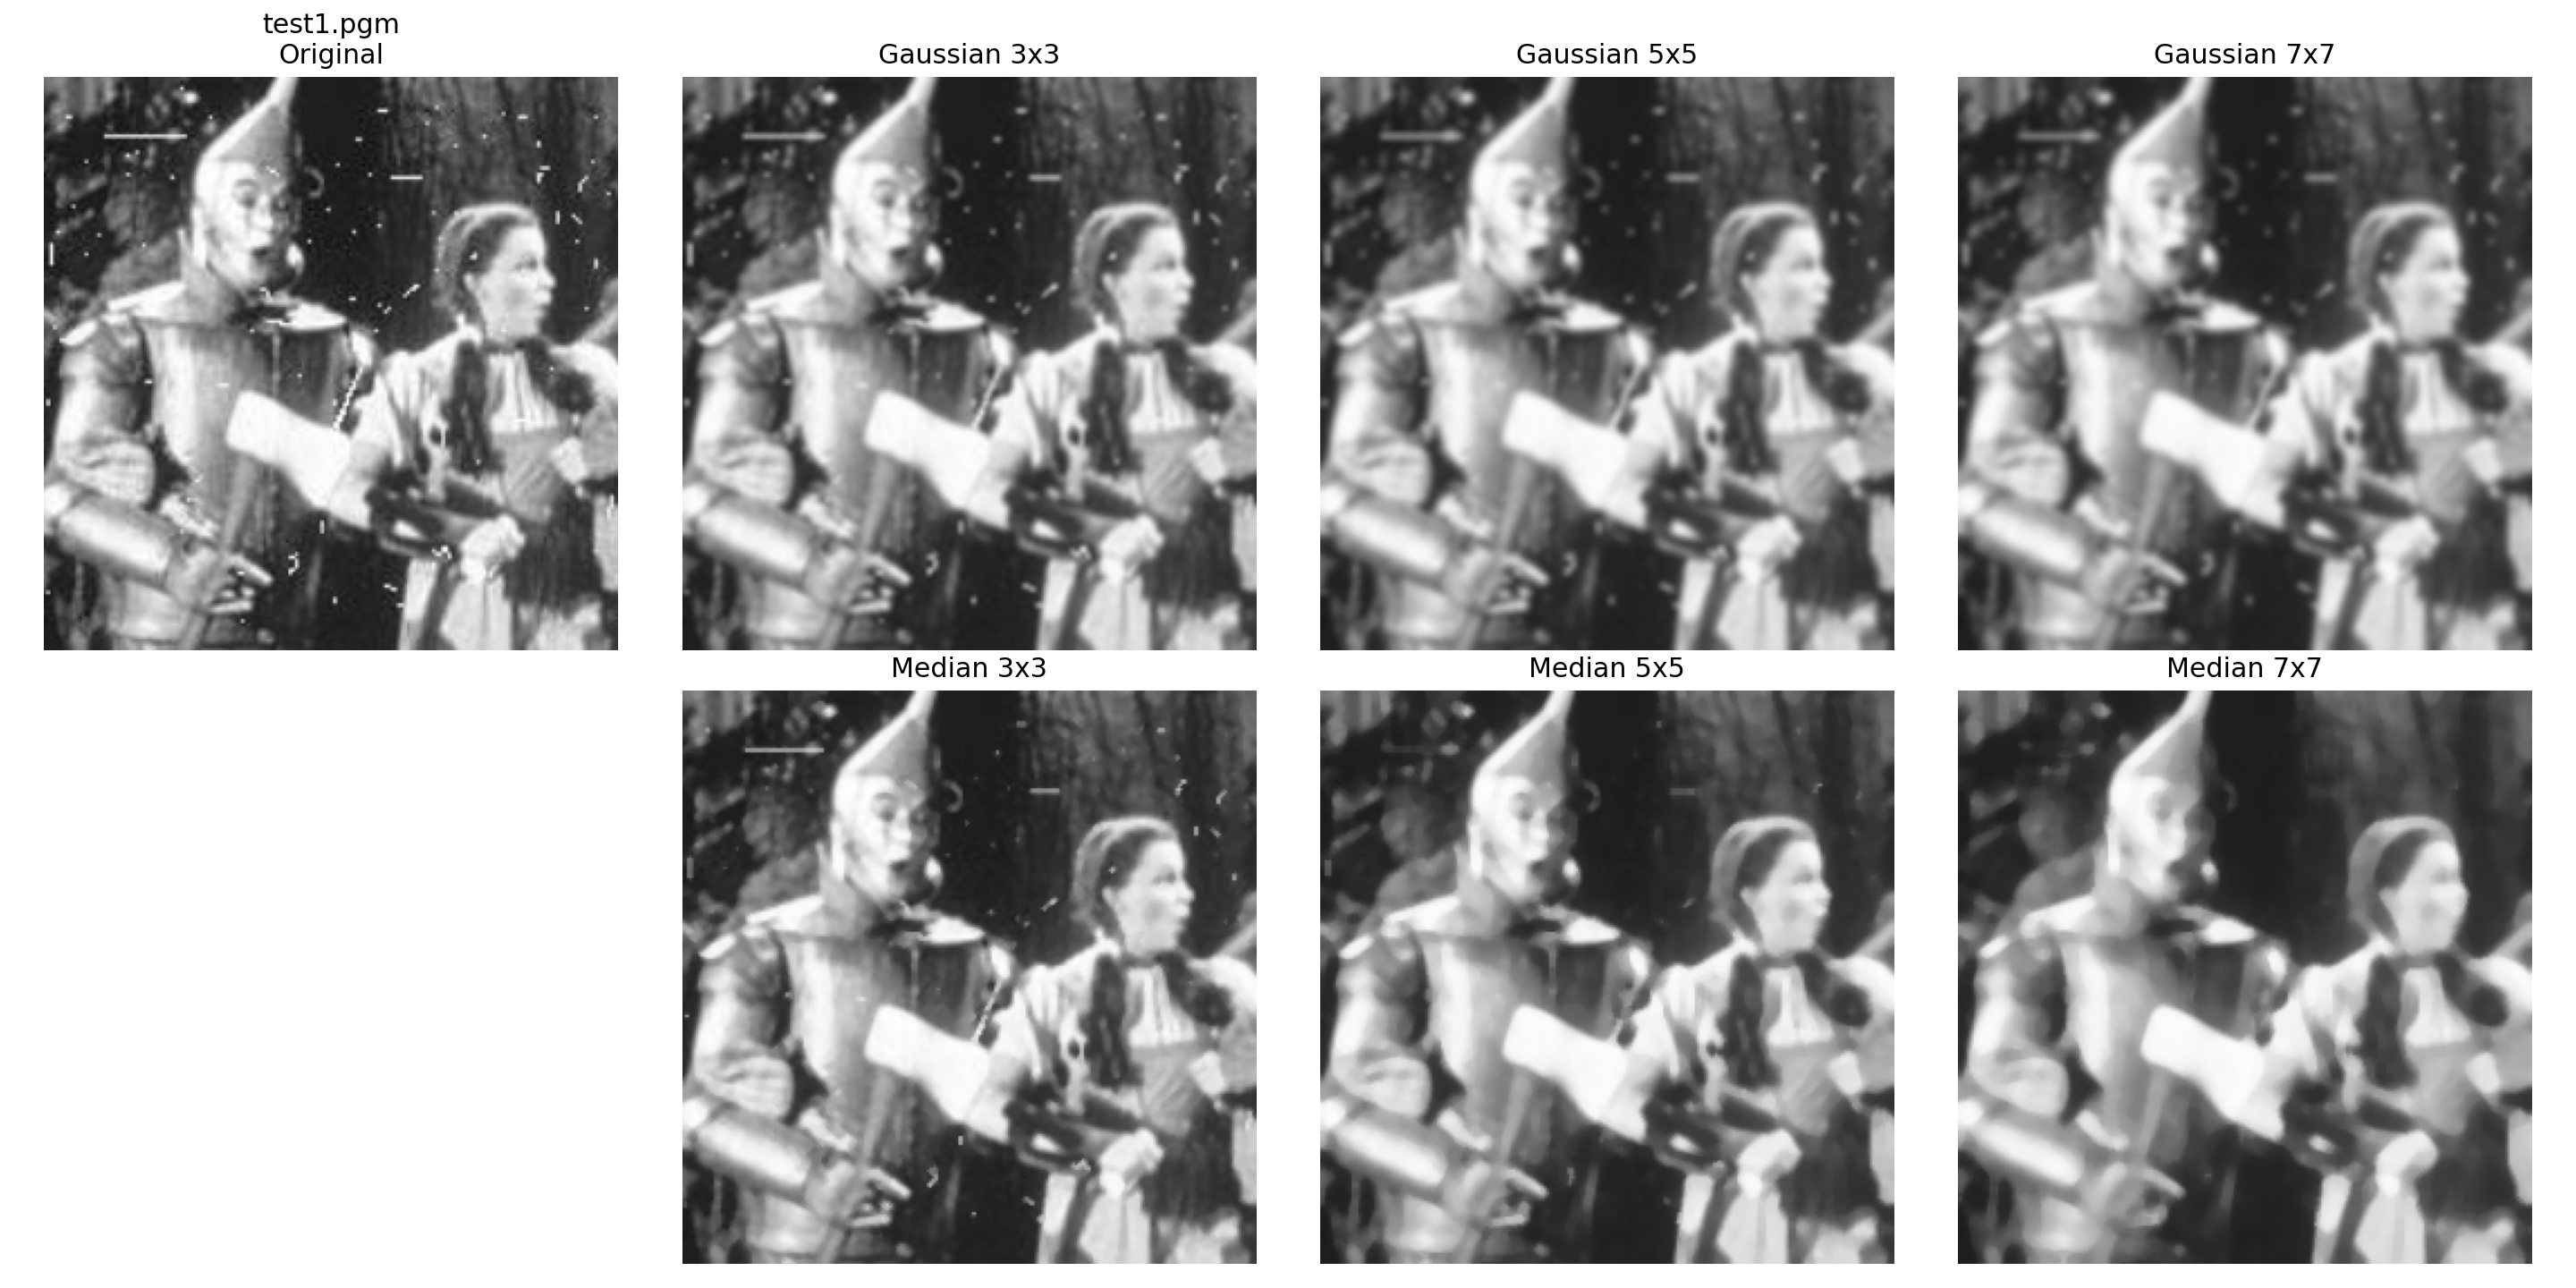
\includegraphics[width=\textwidth]{test1_lowpass_overview.png}
  \caption{\texttt{test1.pgm} 的低通滤波结果总览}
\end{figure}

\begin{figure}[H]
  \centering
  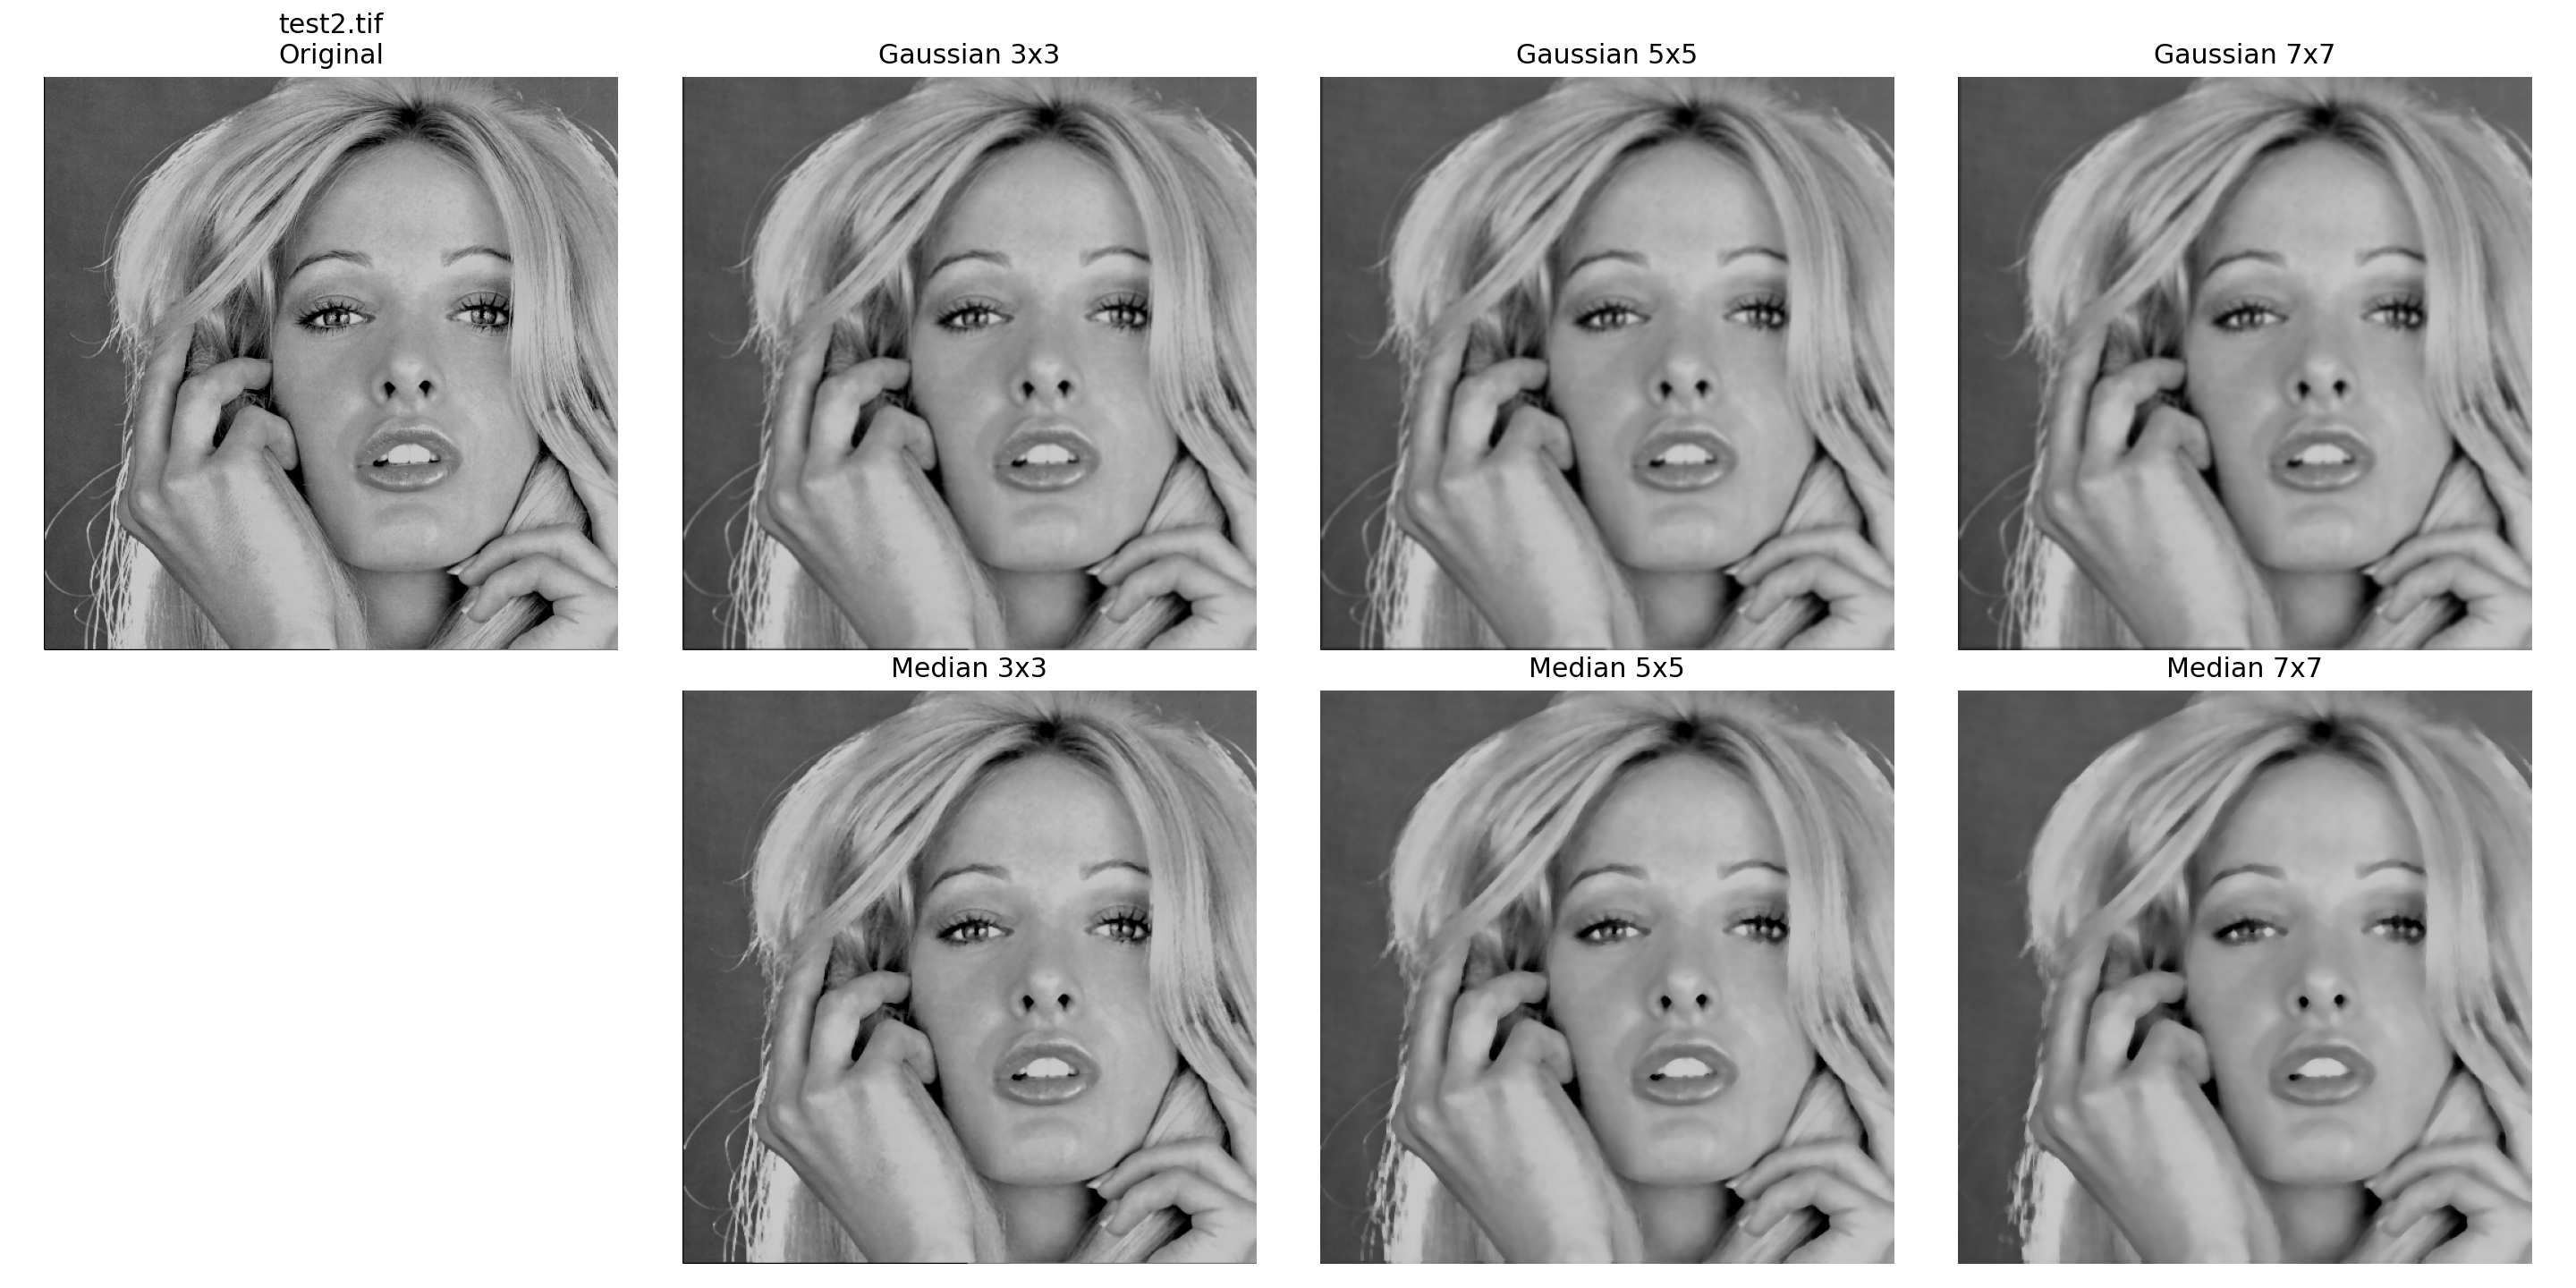
\includegraphics[width=\textwidth]{test2_lowpass_overview.png}
  \caption{\texttt{test2.tif} 的低通滤波结果总览}
\end{figure}

\begin{table}[H]
\centering
\caption{低通滤波指标对比（\texttt{test1.pgm}）}
\begin{tabular}{lccc}
\toprule
方法 & 模板 & gradient\_mean & laplacian\_var \\
\midrule
Original & - & 97.621 & 685.791 \\
Gaussian & $3\times3$ & 82.121 & 122.768 \\
Gaussian & $5\times5$ & 71.789 & 49.634 \\
Gaussian & $7\times7$ & 67.574 & 35.682 \\
Median & $3\times3$ & 82.684 & 309.614 \\
Median & $5\times5$ & 67.668 & 151.655 \\
Median & $7\times7$ & 58.344 & 100.271 \\
\bottomrule
\end{tabular}
\end{table}

\begin{table}[H]
\centering
\caption{低通滤波指标对比（\texttt{test2.tif}）}
\begin{tabular}{lccc}
\toprule
方法 & 模板 & gradient\_mean & laplacian\_var \\
\midrule
Original & - & 55.090 & 1077.965 \\
Gaussian & $3\times3$ & 39.437 & 70.481 \\
Gaussian & $5\times5$ & 32.674 & 19.915 \\
Gaussian & $7\times7$ & 30.478 & 13.424 \\
Median & $3\times3$ & 42.040 & 310.974 \\
Median & $5\times5$ & 30.750 & 112.996 \\
Median & $7\times7$ & 26.038 & 63.664 \\
\bottomrule
\end{tabular}
\end{table}

从结果可以看到，随着模板尺寸从 $3\times3$ 增大到 $7\times7$，两种方法的 \texttt{gradient\_mean} 和 \texttt{laplacian\_var} 都明显下降，说明高频细节不断被抑制，图像越来越平滑。对 \texttt{test1.pgm} 来说，中值滤波对散点型噪声的抑制更直接；对 \texttt{test2.tif} 来说，高斯滤波产生的平滑结果更自然、过渡更连续。

\subsection{高通与边缘检测结果}
\begin{figure}[H]
  \centering
  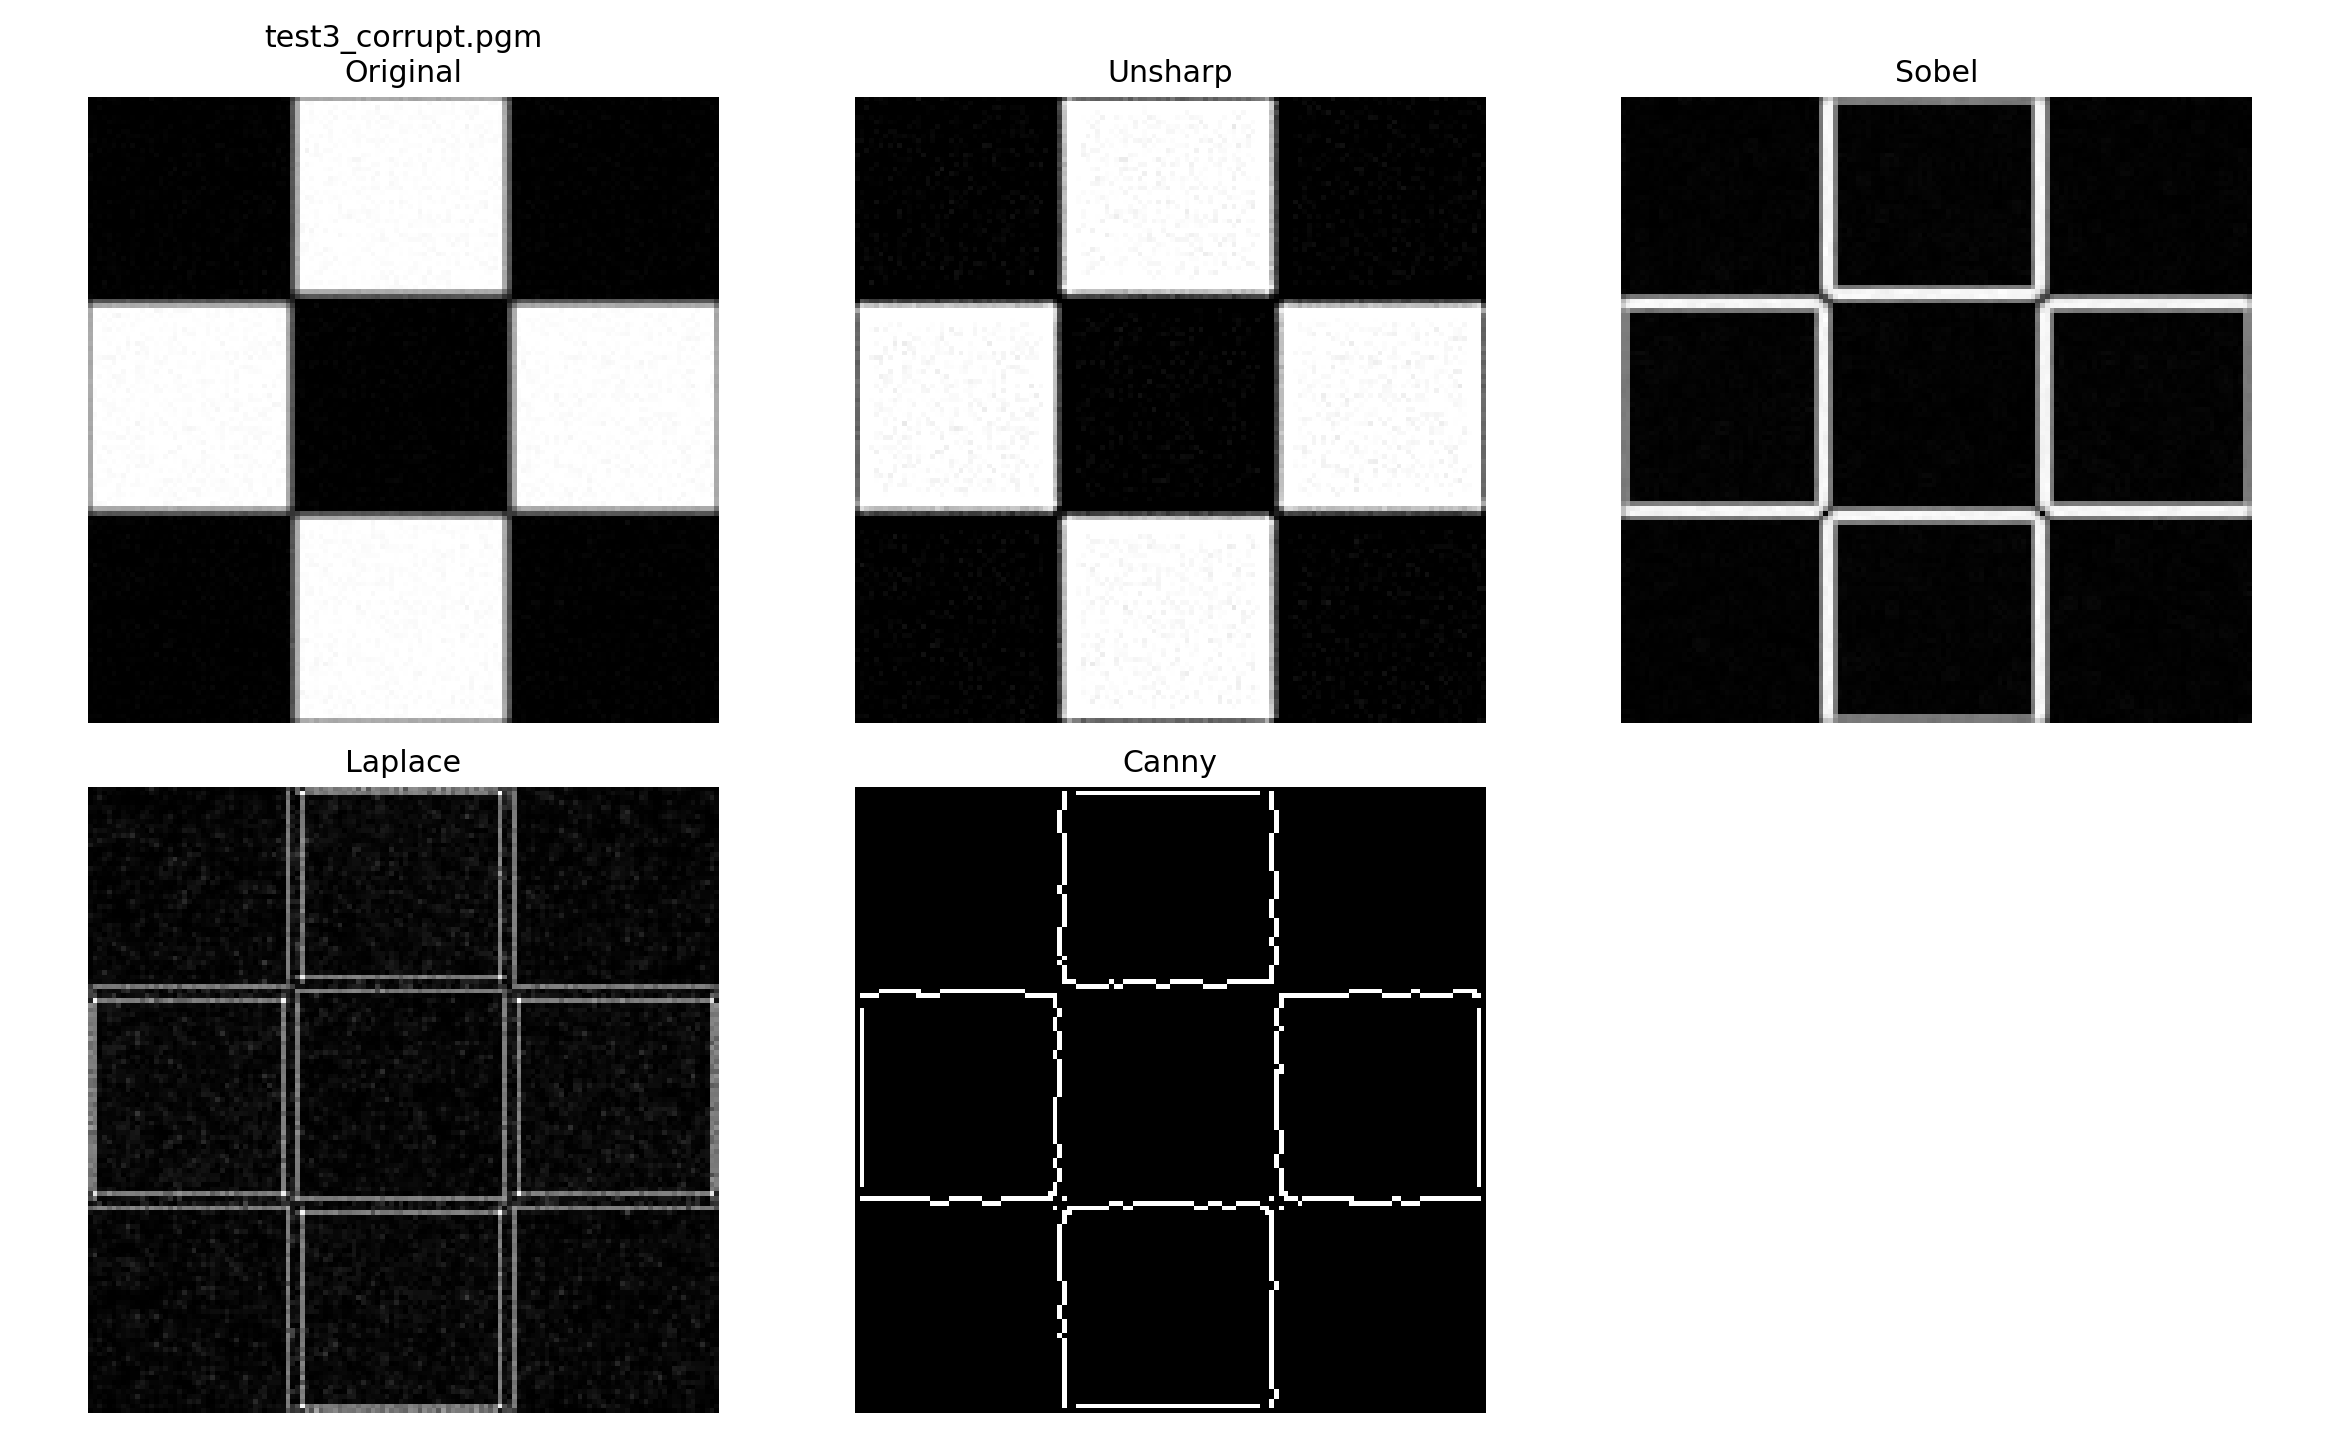
\includegraphics[width=0.95\textwidth]{test3_corrupt_highpass_overview.png}
  \caption{\texttt{test3\_corrupt.pgm} 的高通与边缘检测结果}
\end{figure}

\begin{figure}[H]
  \centering
  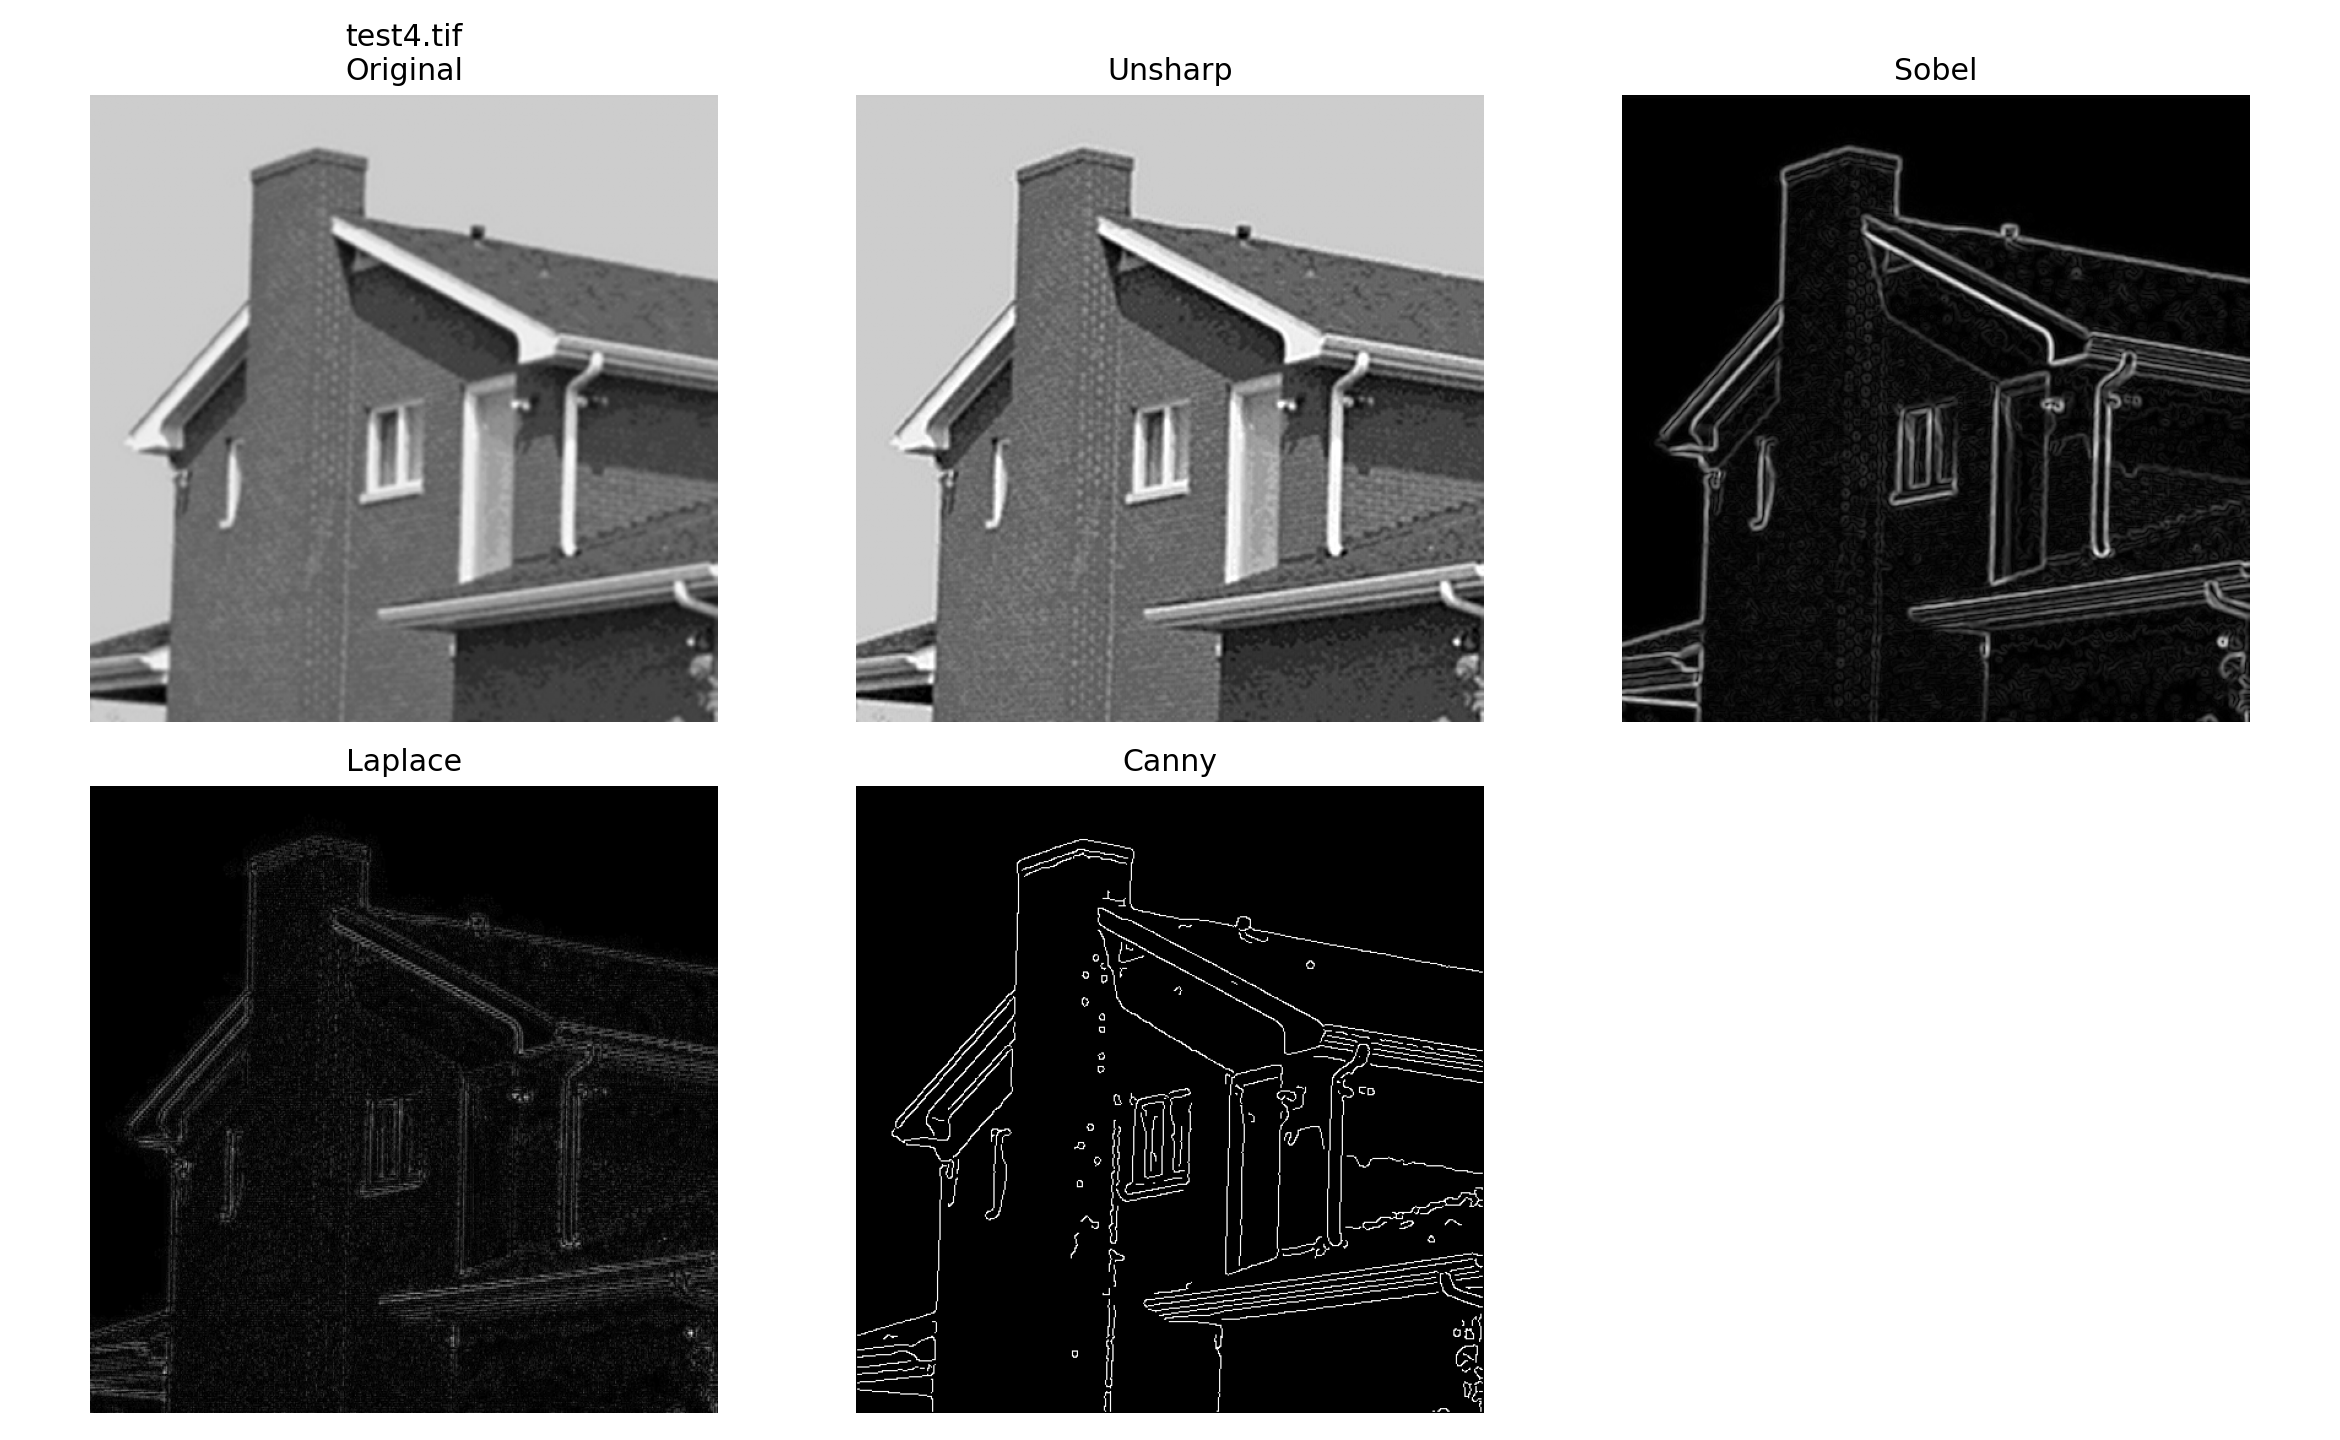
\includegraphics[width=0.95\textwidth]{test4_highpass_overview.png}
  \caption{\texttt{test4.tif} 的高通与边缘检测结果}
\end{figure}

\begin{table}[H]
\centering
\caption{高通与边缘方法指标（\texttt{test3\_corrupt.pgm}）}
\begin{tabular}{lcccc}
\toprule
方法 & mean & std & laplacian\_var & edge\_ratio \\
\midrule
Original & 109.205 & 121.112 & 617.328 & - \\
Unsharp & 108.813 & 121.161 & 1231.188 & - \\
Sobel & 25.260 & 62.747 & 2074.491 & - \\
Laplace & 16.879 & 31.301 & 5484.053 & - \\
Canny & 9.586 & 48.504 & 19928.547 & 0.0376 \\
\bottomrule
\end{tabular}
\end{table}

\begin{table}[H]
\centering
\caption{高通与边缘方法指标（\texttt{test4.tif}）}
\begin{tabular}{lcccc}
\toprule
方法 & mean & std & laplacian\_var & edge\_ratio \\
\midrule
Original & 136.544 & 57.786 & 28.099 & - \\
Unsharp & 136.515 & 59.615 & 113.030 & - \\
Sobel & 17.868 & 29.636 & 336.805 & - \\
Laplace & 11.599 & 15.863 & 1329.777 & - \\
Canny & 9.575 & 48.476 & 20233.992 & 0.0375 \\
\bottomrule
\end{tabular}
\end{table}

从主观视觉上看，Unsharp Masking 更适合做锐化增强，因为它仍保留原始图像外观；Sobel 输出边缘强度图，轮廓清楚但边缘偏粗；Laplace 对细节和噪声都很敏感，轮廓更锐利但也更容易放大干扰；Canny 提取出的边缘最细、最连续，整体可读性最好。

\subsection{优缺点总结}
\begin{table}[H]
\centering
\caption{各方法优缺点总结}
\begin{tabular}{p{2.8cm}p{5.2cm}p{5.2cm}}
\toprule
方法 & 优点 & 缺点 \\
\midrule
Gaussian Filter & 平滑自然，适合抑制高斯型随机噪声 & 会模糊边缘，窗口越大细节损失越明显 \\
Median Filter & 对椒盐噪声、脉冲噪声鲁棒，保边缘能力较强 & 大窗口下容易损失纹理，结果可能偏块状 \\
Unsharp Masking & 适合锐化和增强细节，保持原图视觉结构 & 参数不当会过锐化并放大噪声 \\
Sobel & 简单高效，边缘方向信息明确 & 边缘较粗，对噪声敏感 \\
Laplace & 对细微灰度变化敏感，轮廓增强明显 & 二阶导数放大噪声更严重 \\
Canny & 边缘细、连续性好、抗噪性能较强 & 流程更复杂，依赖参数选择 \\
\bottomrule
\end{tabular}
\end{table}

\section{结论}
\begin{enumerate}
  \item 在低通滤波中，模板越大，平滑效果越明显，但细节和边缘损失也越严重。
  \item 对带有离散噪点的图像，中值滤波通常比高斯滤波更有效；对一般随机噪声，高斯滤波结果更自然。
  \item Unsharp Masking 更适合图像锐化；Sobel、Laplace、Canny 更适合边缘检测。
  \item 在本实验中，Canny 在边缘连续性和清晰度方面表现最好，Laplace 对细节最敏感但也最容易引入噪声响应。
\end{enumerate}

\section*{附：编译与使用说明}
\begin{itemize}
  \item 建议在 Overleaf 选择 \textbf{XeLaTeX} 编译器。
  \item 上传本文件 \texttt{report\_hw4\_overleaf.tex} 与 \texttt{outputs/} 整个文件夹即可。
  \item 本文所有图片都直接来自 \texttt{outputs/task\_lowpass} 和 \texttt{outputs/task\_highpass}。
\end{itemize}

\end{document}
